\documentclass[a4]{article}
\usepackage{geometry}
\geometry{verbose,tmargin=2.5cm,bmargin=2.5cm,lmargin=3cm,rmargin=3cm}
\usepackage{amsmath,amssymb,amsthm}
\usepackage{graphicx}
\graphicspath{{graphics/}}
\usepackage[utf8]{inputenc}
\usepackage{fancyvrb}
\usepackage{hyperref}
\usepackage{lscape}
\usepackage{adjustbox}
\usepackage{verbatim}
\usepackage{subcaption}
\usepackage{gensymb}

\title{MultiFEBE \\ Tutorial 7b: seismic response of a single battered pile}

\author{\'A.G. Vega-Artiles}

\date{March 2023}

\begin{document}

\maketitle

\tableofcontents

\section{Problem description}

In this part b of the seventh tutorial, the seismic response of a single battered pile is obtained. For this purpose, the geometry, mesh and properties from the \textit{Tutorial 7a} for the single battered pile with $\theta=0\degree$ are used. Then, the model was subjected to vertically incident P and SH waves in order to calculate the transfer functions as $I_u=u_g/u_{g_0}$.

\subsection{Input data file}
Solving in MultiFEBE consists of running the software by specifying several options in the following sections\footnote{See reference manual.}: [problem], [settings], [materials], [regions], [conditions over nodes], etc.

The first part to configurate is the problem definition in the section [problem]. This example is a 3D harmonic mechanical problem.

\begin{Verbatim}	
[problem]
n = 3D
type = mechanics
analysis = harmonic
\end{Verbatim}

Then, a list of frequencies is generated by specifying the number of frequencies, that must be $\geq 2$ (20) followed by the minimum frequency $>0$ (0.005976) and the maximum frequency (0.5976), being each one in new lines.

\begin{Verbatim}
[frequencies]
rad/s
lin
20
0.005976
0.5976
\end{Verbatim}

In the section [export], several export and notation settings are defined. In this example, the nodal solutions and the stress resultant solutions will be exported by writing the option F or T with the corresponding expression, ``export\_nso" and ``export\_tot", respectively. Furthermore, the complex notation is set as cartesian and the results for specific nodes are taking by specifying the number of nodes (1) and the identifiers of the nodes (3). 

\begin{Verbatim}
[export]
export_nso = T
export_tot = T
complex_notation = cartesian
nso_nodes = 1 3
\end{Verbatim}

As the problem has two materials, the section [materials] will need three lines: a first line for the number of materials in the model and a line per material with its properties such as tag, type, $\rho$, E, $\nu$ and $ \xi $.

\begin{Verbatim}
[materials]
2
1 elastic_solid rho 1. E 1. nu 0.4 xi 0.05
2 elastic_solid rho 0.428 E 1000. nu 0.25 xi 0.01
\end{Verbatim}

Next step is to configurate the mesh. In this case, a mesh from Gmsh will be used so that it is necessary to write the option number 2 and the document name obtained from it in the section [settings]. However, if the mesh were going to be read from the input file, it would require to write the sections [nodes], [elements] and [parts] instead.

\begin{Verbatim}	
[settings]
mesh_file_mode = 2 "single_pile.msh"
\end{Verbatim}

In the section [boundaries], all boundaries are defined. The first line indicates the number of boundaries (1). Then, one line per boundary indicating the boundary identifier (1), the part identifier that discretizes it (3), and finally the boundary class (ordinary).

\begin{Verbatim}
[boundaries]
1
1 3 ordinary
\end{Verbatim}

In the section [be body loads], all body loads in BE regions are defined. The format consists of a first line with the number of BE body loads to be defined, next as many lines as BE body loads. Each line contains first the BE body load identifier and last the mesh part which contains the elements associated with it.

\begin{Verbatim}
[be body loads]
1
1 1
\end{Verbatim}

The section [fe subregions] indicates the number of fe subregions in the first line (1) and a line per subregions indicating the subregion identifier (1) and the part identifier (2). The last two zeros at the end are mandatory and they are going to be used in the future for additional features.

\begin{Verbatim}
[fe subregions]
1
1 2 0 0
\end{Verbatim}

In the section [cross sections], it is necessary to specify the number of cross sections in the first line and a line per cross section by indicating the type of beam model (strbeam\_eb = straight beam, Euler–Bernoulli model), number of fe subregions related to the cross section (1), fe subregion identifier (1), type of cross section (circle), radius (1.) and reference vector for the section orientation (0. 1. 0.).

\begin{Verbatim}
[cross sections]
1
strbeam_eb 1 1 circle 1. 0. 1. 0.
\end{Verbatim}

The format of the section [regions] consists of a first line indicating the number of regions (2). Furthermore, for each region there must be a block of data consisting of several lines. 

The first region is a BE region, so the first line shows the region identifier and the region class (discretization method) (1 be). The second line indicates the number and list of boundaries (1 1), the third line defines the material (material 1), the fourth line defines the number and list of BE body loads (1 1) and the fifth line the number and list of incident fields (1 1).

The second region is a FE region, so the first line shows the region identifier and the region class (discretization method) (2 fe). Then, the second line indicates the number of subregions (1) and their identifiers (1) and the third line the material (material 2). 

\begin{Verbatim}	
[regions]
2

1 be
1 1
material 1
1 1
1 1

2 fe
1 1
material 2
\end{Verbatim}

In the section [incident waves], the incoming waves are defined. The general format has a first line for the number of waves (1), a second line for the wave identifier (1), a third line for the wave class (plane), a fourth line for the space (half-space with $np = 3$, $xp = 0$, $bc = 1$), a fifth line for the variable (0 for displacement), the amplitude (1.,0.), the reference point ($ x0(1) = 0 $, $ x0(2) = 0 $, $ x0(3) = 0 $) and the angles ($ varphi = 0 $, $ theta = 0 $), a sixth line for symmetry options ($ xs(1) = 0 $, $ xs(2) = 0 $, $ xs(3) = 0 $, $ symconf(1) = 0 $, $ symconf(2) = 0 $, $ symconf(3) = 0 $) and a seventh line for the region type (viscoelastic) and the wave type (p).

\begin{Verbatim}	
[incident waves]
1
1
plane
half-space 3 0 1
0 (1.,0.) 0. 0. 0. 0. 90.
0. 0. 0. 0. 0. 0.
viscoelastic p
\end{Verbatim}

The whole data file applied to the problem is the following:

\begin{Verbatim}
[problem]
n = 3D
type = mechanics
analysis = harmonic

[frequencies]
rad/s
lin
20
0.005976
0.5976

[export]
export_nso = T
export_tot = T
complex_notation = cartesian
nso_nodes = 1 3

[materials]
2
1 elastic_solid rho 1. E 1. nu 0.4 xi 0.05
2 elastic_solid rho 0.428 E 1000. nu 0.25 xi 0.01

[settings]
mesh_file_mode = 2 "single_pile.msh"

[boundaries]
1
1 3 ordinary

[be body loads]
1
1 1

[fe subregions]
1
1 2 0 0

[cross sections]
1
strbeam_eb 1 1 circle 1. 0. 1. 0.

[regions]
2
1 be
1 1
material 1
1 1
1 1

2 fe
1 1
material 2

[incident waves]
1
1
plane
half-space 3 0 1
0 (1.,0.) 0. 0. 0. 0. 90.
0. 0. 0. 0. 0. 0.
viscoelastic p
\end{Verbatim}

\section{Results and discussion}

Figures \ref{fig:p-wave} and \ref{fig:sh-wave} show the transfer functions for a single battered pile. 

\begin{figure}[tbh!]
	\centering
	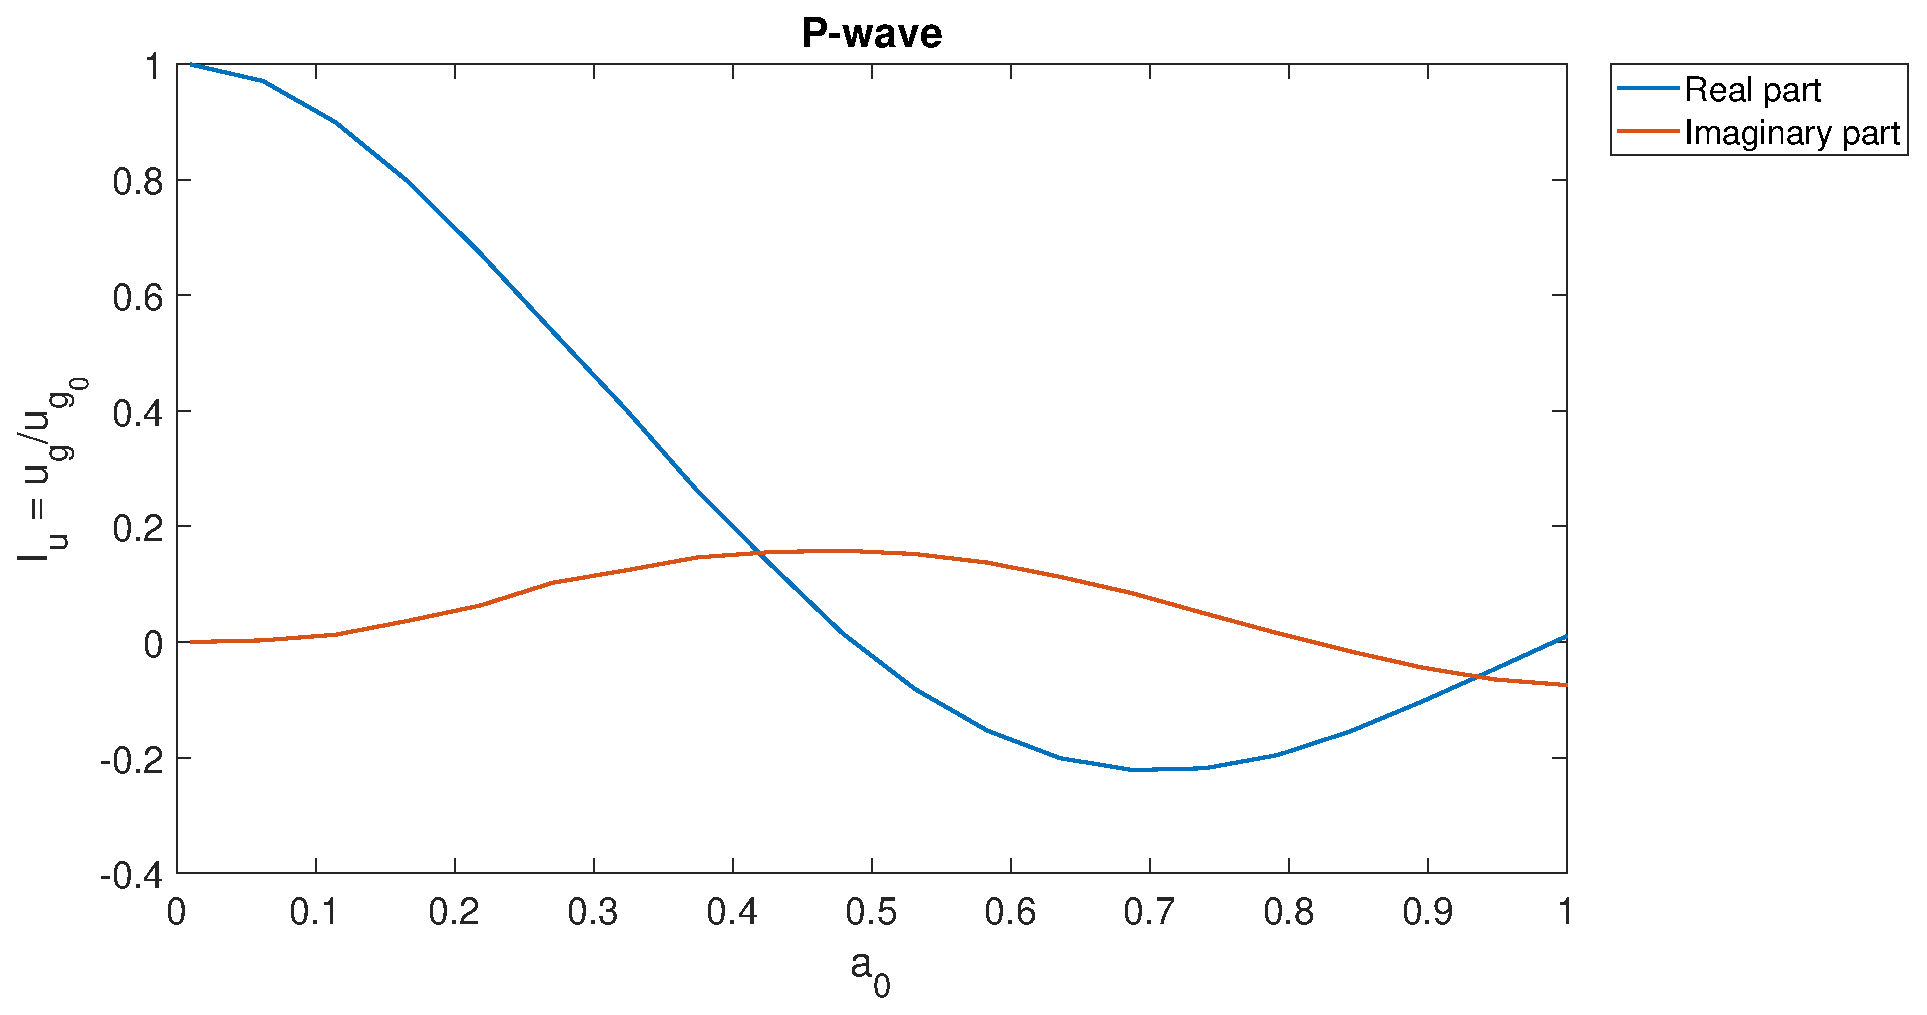
\includegraphics[scale=0.5]{p-wave.eps}
	\caption{Transfer function for a single battered pile subjected to a vertically incident P-wave.}
	\label{fig:p-wave}
\end{figure}

\begin{figure}[tbh!]
	\centering
	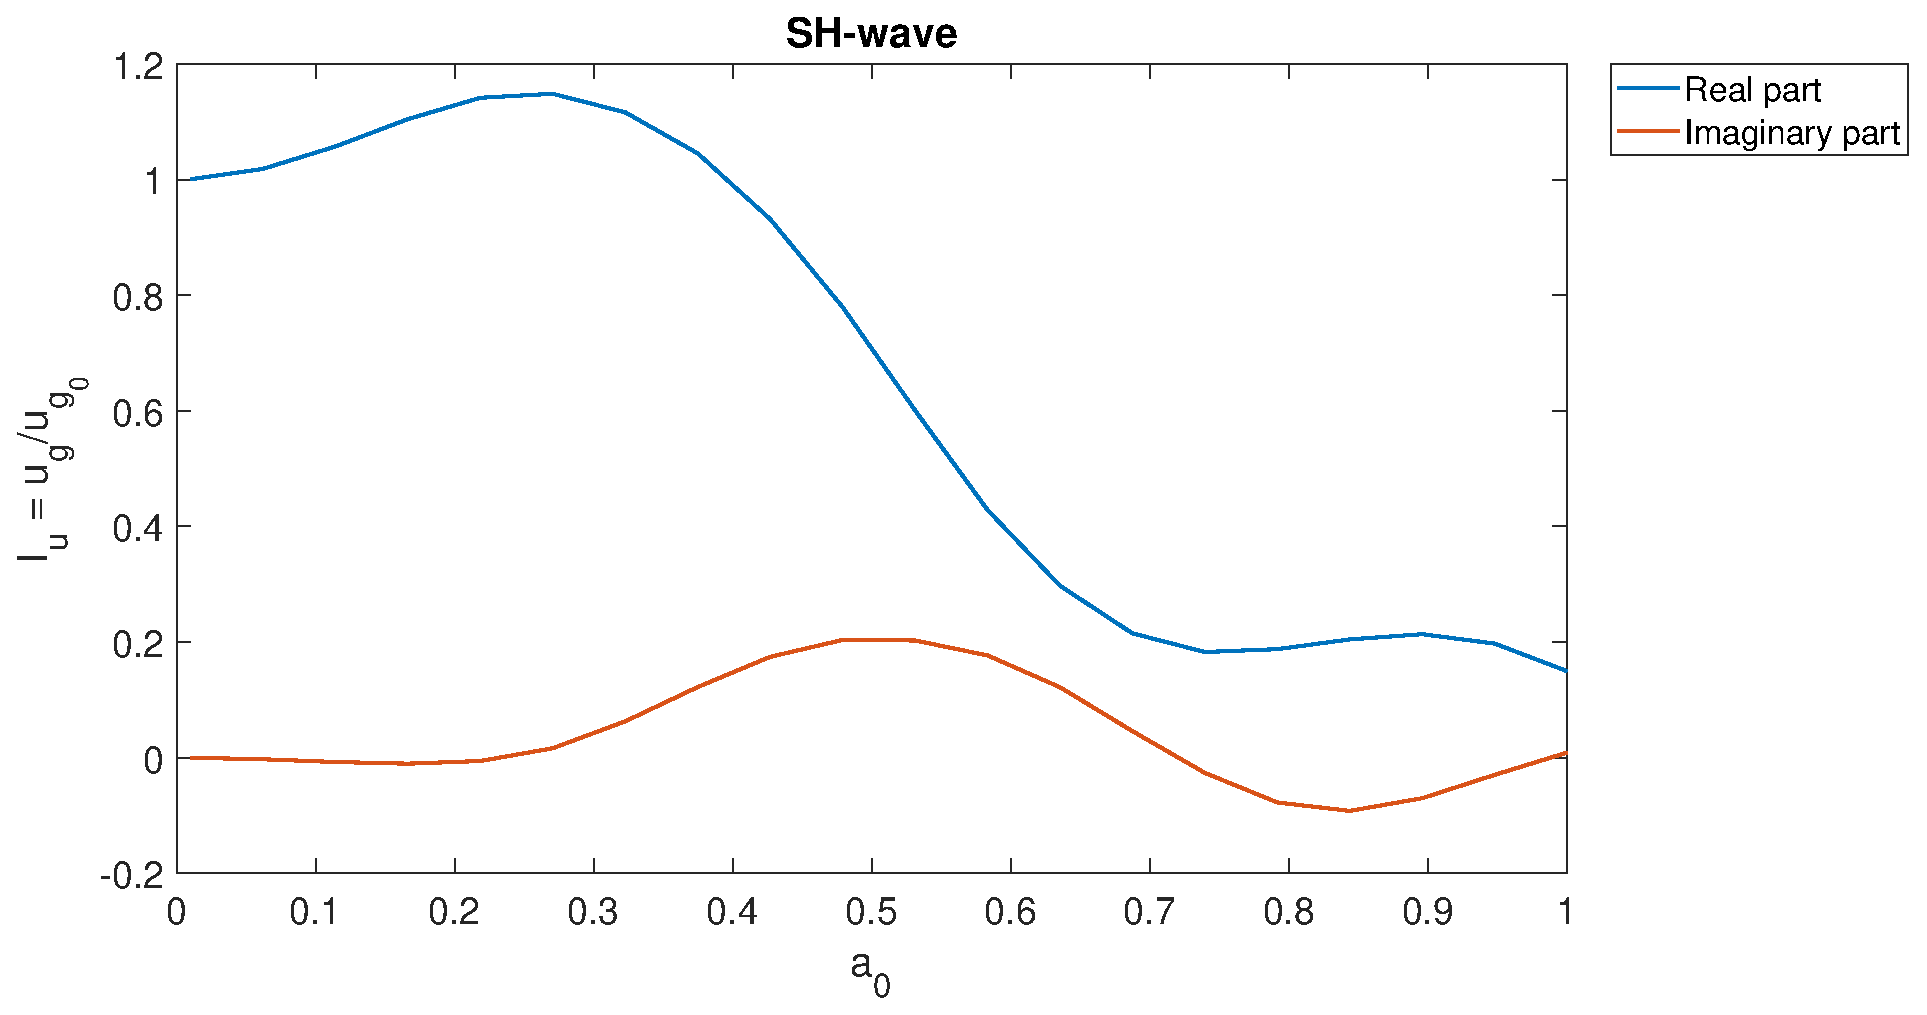
\includegraphics[scale=0.5]{sh-wave.eps}
	\caption{Transfer function for a single battered pile subjected to a vertically incident SH-wave.}
	\label{fig:sh-wave}
\end{figure}

\end{document}
